\documentclass[a4paper]{article}

%% Language and font encodings
\usepackage[english]{babel}
\usepackage[utf8x]{inputenc}
\usepackage[T1]{fontenc}
\usepackage{siunitx}
%% Sets page size and margins
\usepackage[a4paper,top=3cm,bottom=2cm,left=3cm,right=3cm,marginparwidth=1.75cm]{geometry}

%% Useful packages
\usepackage{amsmath}
\usepackage{graphicx}
\usepackage{verbatim}
\usepackage[colorinlistoftodos]{todonotes}
\usepackage[colorlinks=true, allcolors=black]{hyperref}

\title{Project Planning}
\author{Software Engineering 2}
\date{January 22,2017}
%--------------------
%Table settings
% % CUSTOM COMMANDS

% Allow lstinline to break long word
\makeatletter%
\def\lst@lettertrue{\let\lst@ifletter\iffalse}%
\makeatother%

% Commands to insert a code line or a reference to code inside text.
\usepackage{color}
\definecolor{inlinecode}{rgb}{0,0.298,0.6}
\newcommand{\code}[1]{%
	\lstinline[
	breaklines=true,
	breakatwhitespace=false, % if true, allow line breaking only after a white space
	%prebreak=-, % insert an hypern when a word is broken on two lines
	basicstyle=\ttfamily\color{inlinecode},
	stringstyle=\color{inlinecode},
	]|#1|}
\newcommand{\checklist}[1]{\textbf{C#1}}
\newcommand{\codeline}[1]{\textsf{L.#1}}
\newcommand{\codelines}[2]{\textsf{L.#1-#2}}

% Marginal note for observations
\newcommand{\note}[1]{\MakeUppercase{#1}\marginpar{\MakeLowercase{\textcolor{red}{#1}}}}

% Test table
\newenvironment{testtable}{
	\begin{longtable}{|p{\dimexpr.35\textwidth}|p{\dimexpr.55\textwidth}|}
}{
	\end{longtable}
}

% FP table
\newenvironment{fptable}[2]{
	\begin{center}
	#1
	\begin{longtable}{|c|c|c|c|}
	\hline 
	&
	\multicolumn{3}{|c|}{{#2}}\\\nopagebreak\hline	
}{
	\hline\end{longtable}\end{center}
}

% FP count table
\newenvironment{fpcounttable}[1]{
	\begin{center}
	\begin{longtable}{|l|l|l|}
	\hline 
	#1 & Complexity & FPs \\\hline
}{
	\end{longtable}\end{center}
}

\newenvironment{fptotaltable}{
	\begin{center}
	\begin{longtable}{|l|r|}
	\hline 
	Function Type & Value \\\hline
}{
	\end{longtable}\end{center}
}

\newcommand{\fptotal}[1]{
	\multicolumn{2}{|l|}{{Total}}
	& #1\\\hline
}

\newcommand{\fpproduct}[1]{
	\multicolumn{2}{|l|}{{Product}}
	& #1\\\hline
}

%  table
\newenvironment{scaledriverstable}[1]{
	\setlength{\LTleft}{-40pt}
	\begin{center}
	#1 
	\begin{longtable}{|p{\dimexpr.16\textwidth}|p{\dimexpr.14\textwidth}|p{\dimexpr.14\textwidth}|p{\dimexpr.14\textwidth}|p{\dimexpr.14\textwidth}|p{\dimexpr.14\textwidth}|p{\dimexpr.14\textwidth}|}
	\hline
}{
	\hline\end{longtable}\end{center}
}

% scale driver count table
\newenvironment{factorcounttable}[1]{
	\begin{center}
	\begin{longtable}{|l|r|r|}
	\hline 
	#1 & Factor & Value \\\hline
}{
	\end{longtable}\end{center}
}

%  table
\newenvironment{costdriverstable}[1]{
	\setlength{\LTleft}{-40pt}
	\begin{longtable}{|p{\dimexpr.16\textwidth}|p{\dimexpr.14\textwidth}|p{\dimexpr.14\textwidth}|p{\dimexpr.14\textwidth}|p{\dimexpr.14\textwidth}|p{\dimexpr.14\textwidth}|p{\dimexpr.14\textwidth}|}
	\hline
	\multicolumn{7}{|c|}{{#1}}\\\hhline{|=======|}
}{
	\hline\end{longtable}
}

\newcommand{\costdescriptors}[7]{
	#1 & #2 & #3 & #4 & #5 & #6 & #7\\
}

\newcommand{\ratinglevel}[6]{
	Rating level & #1 & #2 & #3 & #4 & #5 & #6 \\\hline
}

\newcommand{\effortmultipliers}[6]{
	Effort multipliers & #1 & #2 & #3 & #4 & #5 & #6 \\\hline
}


\newcommand{\addfactor}[7]{
	#1 & #2 & #3 & #4 & #5 & #6 & #7 \\
}
\newcommand{\addfactorvalues}[6]{
SF$_j$ & #1 & #2 & #3 & #4 & #5 & #6 \\\hline
}

	


% Methods in test tables
\newcommand{\method}[1]{%
	\nopagebreak
	\multicolumn{2}{|c|}{{#1}}\\\nopagebreak\hline
	\textit{Input} & \textit{Effect}\\\nopagebreak\hline
}


\newcommand{\fpvalues}[4]{%
	\textit{#1} & \textit{#2}& \textit{#3}& \textit{#4}\\\nopagebreak\hline
}
	
	
% Double horizontal line for test table
\newcommand{\dline}{\nopagebreak\hhline{|==|\nopagebreak}}
\usepackage{longtable}
\usepackage{hhline}
\usepackage{floatflt}
%---------------------
\begin{document}
\maketitle

\begin{figure}[h]
  \centering
  
\includegraphics[width=300 pt]{resources/polimi.png}
  \label{fig:polimi}
\end{figure}

\emph{\\}
\emph{\\}
\emph{\\}
\emph{\\}
\emph{\\}
\emph{\\}
\emph{\\}
\emph{\\}
\emph{\\}
\emph{\\}

\begin{minipage}{0.7\textwidth}
\begin{flushleft} \large
\emph{Authors:}\\
Claudio Salvatore \textsc{Arcidiacono} Matr 879109\\
Antonio \emph{ }\emph{ }\emph{ }\emph{ }\emph{ }\emph{ }\emph{ }\emph{ }\emph{ }\emph{ }\emph{ }\emph{ }\textsc{Di Bello} \emph{ }\emph{ }\emph{ }\emph{ } Matr 878786\\
Denis  \emph{ }\emph{ }\emph{ }\emph{ }\emph{ }\emph{ }\emph{ }\emph{ }\emph{ }\emph{ }\emph{ }\emph{ }\emph{ }\emph{ }\emph{ }\textsc{Dushi } \emph{ }\emph{ }\emph{ }\emph{ }\emph{ }\emph{ }\emph{ }\emph{ }\emph{ }Matr 879115
\end{flushleft}
\end{minipage}

\begin{minipage}{0.4\textwidth}

\end{minipage}

\pagenumbering{gobble}
\newpage
\pagenumbering{arabic}

\tableofcontents

\newpage
\section{Introduction} 

\subsection{Description of the given problem}
We will project and implement PowerEnJoy, which is a digital management system for a car-sharing service that exclusively employs electric cars.
The system that will be developed has to allow users to register and log in to the service, to see which car are available and were the cars can be parked. In addition to the basic functionality of a car-sharing service the system has to incentive virtuous behaviors of the users, like plugging the car to a charging station or leaving the car with enough charge, in order to have as much as possible a self-sustainable service.

\subsection{Goals}

\begin{itemize}
\item [G1]A client can register to the system by providing an e-mail, valid payment information and a photo of his driving license.

\item [G2]A client can log in to system.

\item [G3]Allows clients to obtain information about available cars(position and remaining charge), safe areas(boundaries) and charging stations (position and available plugs).

\item [G4]Allows clients to reserve a car that fits most their needs.

\item [G5]A client can start the rent opening a car that has reserved previously when he/she is in the near by.

\item [G6]During the rent a client can display the amount of money charged.

\item [G7]Guarantee as many available cars as possible encouraging clients to have a virtuous and eco-friendly behavior applying fees and discounts.

\item [G8]Allows clients to end the rent and leave the car in any safe area.

\item [G9]Clients can report eventual damages made by users that have driven the car before.

\item [G10]Clients can set the money saving option.


\end{itemize}


\subsection{Domain assumption}
We suppose that these properties hold in the analyzed world :
\begin{itemize}
\item All cars have a stable GPS signal.
\item Clients shares their position when they use the application.
\item PowerEnJoy always has updated data about all the cars and the power stations.
\item The power grid always guarantees electric power.
\item The only method to enter in a car is by the doors.
\item The company cars have at least 4 seats.
\item The streets are correctly mapped in the system.
\item All cars have stable internet connection.
\item The charging sensor reflects the real charge of the car in real-time.
\item The real charge of parked cars stays the same over time. 
\item Charging stations are not in the same GPS position.
\item There aren't two clients with the same  personal data.
\end{itemize}

\newpage

\subsection{Glossary}
\textbf{Guest:}
 is an user that is not registered yet to PowerEnJoy.\\
\textbf{Client:}
is an user that has completed successfully the registration procedure.\\
\textbf{Logged client:}
is a client that has logged into PowerEnJoy.\\
\textbf{Blocked client:}
is a client that is not allowed to log in to system because he has some debits with PowerEnJoy.\\
\textbf{User:}
a client or a guest.\\
\textbf{Virtuous  behavior:}
the client has a "Virtuous behavior" if he performs one or more of the following actions: 
\begin{itemize}
\item transport at least other two passengers into the car.
\item leaves the car with less than 50\% of the battery empty.
\item plugs the car into the power grid of a charging station.
\end{itemize}
\emph{\\}
\textbf{Rent:} defines the period of time that starts when the logged client opens the car and ends when the door of the car are locked due to a "end rent" request of the logged client.\\
\textbf{Pin:} a personal sequence of four numbers given by the system after the registration, necessary to start the engine.\\
\textbf{Map Information:}
denotes the following information: 
\begin{itemize}
\item location of available cars.
\item location of charging areas.
\item for each charging area the number of available charging spots.
\item boundaries of safe areas.
\end{itemize}
\emph{\\}
\textbf{Not valid data:}
syntactically incorrect data (e.g. mail not in the format local-part@domain).\\
\textbf{Credentials:}
email and password used to log into PowerEnJoy.\\
\textbf{Valid Credentials:}
email and password related to a registered user.\\
\textbf{Car information Menu:}
displayed when a client selects a car on the map. In this menu are displayed the information about the car (remaining charge percentage and license plate number) and a button that can be used to reserve the car.\\
\textbf{Safe Areas:} 
areas in which is permitted to the client to end the rent and leave the car.\\
\textbf{Valid Payment Information:}Credit or prepaid card with at least a minimum amount of money.\\

\subsection{Synonymous}
\begin{itemize}
\item rental: rent 
\item charging area: charging station
\item client : logged client. Sometimes an action can be performed only by a client that has logged previously. We will use client instead of logged client when this distinction is not ambiguous.
\end{itemize}

\subsection{Interfaces to external applications}
The PowerEnJoy system interacts with the following external systems:
\begin{itemize}
\item \textbf{Operators system:} to share with operators information about the rental chronology, the cars position, remaining charge and  reports of damaged/dirty car for maintenance and legal purposes. 
\item  \textbf{Civil registry office:} to obtain user profile information from ID number.
\item \textbf{Transport authority:}  to obtain user profile information from license number.
\item \textbf{Payment gateway:} to verify the validity of the payment information and to charge the clients. 
\end{itemize}


\subsection{Reference Documents}
\begin{itemize}
\item Specification Document: Assignments AA 2016-2017.pdf
\item  IEEE Std 830-1998 IEEE Recommended Practice for Software Requirements
Specifications.
\item  Examples documents:  
\begin{itemize}
\item MeteoCal RASD example2.pdf
\item RASD sample from Oct. 20lecture.pdf 
\end {itemize}
\end {itemize}

\newpage
\section{Project size, cost and effort estimation}
In the section below we will use function points and COCOMO II approaches in order to provide an estimation of the expected size, cost and required effort for \textbf{PoweEnJoy}.



\subsection{Size estimation: function points}
The size estimation will be estimated using the \textbf{Function Points} approach, spotting at first what are the main functionalities of our system and how many lines of code we aspect to be written in JEE. According to the function points approach, the LOC can be estimated using the following formula:

\begin{center}
$LOC =  FP \cdot AVC $
\end{center}

where:
\begin{itemize}
\item LOC = Lines of code
\item FP = Function Points
\item AVC = language specific constant, for JEE is between 46 for an lower bound and 67 for an upper bound
\end{itemize}
In order to estimate the overall function points, this approach needs a first classification of our main files into 2 categories: 
\begin{itemize}
\item Internal Logic files : homogeneous set of data used and managed by the application .
\item External Interface files:homogeneous set of data used by the application but generated and maintained by other applications.
\end{itemize}
and a classification of the main functionalities into 3 main categories:
\begin{itemize}
\item External Input: Elementary operation to elaborate data coming from the external environment.
\item External Output:Elementary operation that generates data for the external environment.
\item External Inquiry:Elementary operation that involves input and output, Without significant elaboration of data from logic files.
\end{itemize}
Once we have identified  the most relevant functions of our system, we attribute a  complexity to each of them and based on the category to which it appertain we  assign some function points.
The function points have been obtained from statistical studies of past projects.
The  weights that we will use for each category will be:\\
\begin{center}
\begin{tabular}{ c c c c  }
\hline
 &\multicolumn{3}{ c }{Complexity Weight} \\\hline
 \textit{Function Type} & \textit{Low}&\textit{Average}&\textit{High}\\\hline
 Internal Logic Files & 7 & 10&15\\
External Interface Files & 5 & 7&10\\
External Input & 3& 4&6\\
External Output & 4& 5&7\\
External Inquiries & 3& 4&6\\

\hline

\end{tabular}
\end{center}
\newpage
\subsubsection{Internal Logic Files (ILF)}
PowerEnJoy need to stores a big amount of data about users, cars and his  assets, so it will use several ILFs. Here below we will see in detail the most relevant.
\begin{itemize}

\item First of all the system will store data about its users (name, surname, email, address, fiscalcode, driving license code and picture ,  ID number, cellphone number) and since this entity will have several attributes  and it will contain around 200.000 entries (considering that the system will run in a city like Milan, where other competitors have similar numbers) we can attribute to this ILF an \textbf{Average} complexity.\\
\item For each client  the system will store data about his payment information, but since this entity has few attributes and it is related 1 to 1  just with the client data, and since these data will be inserted and uploaded rarely we can consider its complexity as \textbf{Low}.\\
\item For each client we will need to store his login data, for the same reasoning as above we will consider this entity complexity as \textbf{Low}.\\
\item The main function of our system is to allow users to reserve and rent cars so the main data that we will store will concern reservations and rents. Assuming that an average client will do 4-5 rents we estimate that the system must be able to store 800.000 - 1M entries. During the day there are some hours were our users will use the system more than during others so we will have a huge traffic of insert and delete that our system must be able to handle in parallel. Furthermore this entities are linked with a lot of other structures in our system so, given the nature of them we can estimate  their complexity as \textbf{High}.\\
\item The system also need to store information about cars, an entity that will be updated pretty often and that has several relations with other structures; but we assume that the system will handle between few hundreds and a thousand cars (so entries); compared with other entities they aren't that much, so  we can estimate the complexity of the ILF as \textbf{Low}.\\
\item The system has to provide a map that will contain information about cars,  were to park them and where to charge them so it has to store information about safe areas and charging stations.  Since these two entities contain few entries (around one hundred charging stations and  tens of safe areas) and that these tables will not be updated very often we can consider their complexity as \textbf{Low}.\\
\end{itemize}
The overall estimation for ILF is summarized in the following table:
\begin{center}
\begin{tabular}{|l l l|}
\hline
\multicolumn{1}{|c}{ILF}&Complexity&FPs\\
\hline
Clients data & Average & 10\\
Payment Information data & Low & 7\\
Login data &Low&7\\
Reservations & High & 15\\
Rents & High&15\\
Cars & Low & 7\\
Safe Areas & Low& 7 \\
Charging Stations & Low & 7\\\hline
\multicolumn{2}{|c}{Total}&75\\
\hline
\end{tabular}
\end{center}
\newpage

\subsubsection{External Interface Files (EIF)}
The external interface files  that the system relies on are the one coming from the external interfaces: the  transport authority, the civil registry and the payment gateway. The system communicates also with an external interface to the operator system but since there are no input data from that interface we will not consider it. Here we will analyze the three EIFs:
\begin{itemize}
\item During the registration phase the user has to input his driving license number; this data is used to call an external service provided by the transport authority and to verify that the driving license is valid for our purpose. This is an operation that happens rarely (once per client) and that involves only one structure ( client data ) using only one request, so we can consider this EIF as a \textbf{Low} complexity one. \\
\item  During the registration phase the user has to input his ID number, this data is used to call an external service provided by the civil registry  to verify the validity of the data inserted. As the one above this operation happens rarely (once per client) and involves only one structure ( client data ) using only one request, so we can consider this EIF as a \textbf{Low} complexity one. \\ 
\item After that a client has ended the rent the system start the payment process throw the payment gateway. From this process we acquire the receipts for the payment that has to be stored. Since this operation will take place pretty often and since these are sensible data and for this reason have to be stored in an high security data structure we can consider this EIF as an \textbf{High} complexity one.
\end{itemize}
Summarizing this function we can derive the following table:
\begin{center}
\begin{tabular}{|l l l|}
\hline
\multicolumn{1}{|c}{EIF}&Complexity&FPs\\
\hline
Driving License & Low& 5 \\
Personal Data & Low & 5\\
Payments Data& High&10\\\hline
\multicolumn{2}{|c}{Total}&20\\
\hline
\end{tabular}
\end{center}
\subsubsection{External Inputs(EI)}
The PowerEnjoy system has to interact with our clients for different purposes (In order to understand the complexity of these functions we will refer often to the components described in the components diagram of the design document):
\begin{itemize}
\item \textbf{Login/Logout:} This is an operation that requires only a component (UserController) and just with one entity, so we can classify this function as a \textbf{Low} complexity one.
\item \textbf{Registration:} This operation requires one component and the interaction with two external interfaces so we can estimate its complexity as \textbf{Average}.
\item \textbf{Reservation Request:} This operation requires the cooperation of a few components; we will have to verify if the car is available (CarController), if so we have to insert the reservation in the database, modify the status of the car (CarRemoteController and CarController) and send the feedback to the user so we can estimate its complexity as \textbf{Average}.
\item \textbf{Cancel Reservation:} This operation requires the same components as the one before so reasoning in the same way we can estimate its complexity as \textbf{Average}.
\item \textbf{Report Damaged Car:} This operation requires a complex function in the CarRemoteController that has to interact with the server system (using CarController) and then communicate with the operator system using an external interface, so given the number of components and the interaction throw an external interface we can estimate its complexity as \textbf{High}.
\item \textbf{Start rent:} this operation requires the cooperation of quite all the components of our system and it has to query the database changing the status of the rent and the reservation, so we can estimate this operation as an \textbf{High} complexity function.
\item \textbf{End rent:} This operation requires the cooperation of a lot of components: CarController for the car position, CarController to change the status of the car and check if the car is plugged, RentController to check information about the rent and others. It also has to start the payment process throw an external interface and it has to query the database to update the rent data. We can consider it an \textbf{High} complexity function.
\item \textbf{Pin Insertion:} After that a client enters in a car and wants to start the engine he has to authenticate  himself inserting the pin in the car system. This operation is just a simple check that  requires the cooperation of few components(CarController, CarRemoteController) and a query in the database. It also has to use an high security protocol so we can say that the complexity of this function is \textbf{Average}
\end{itemize}

Summing up all the function spotted we derive the following table:
\begin{center}
\begin{tabular}{|l l l|}
\hline
\multicolumn{1}{|c}{EI}&Complexity&FPs\\
\hline
login/logout & Low & 2x3\\
Registration & Average & 4\\
Reservation Request &Average&4\\
Cancel Reservation & Average&4\\
Report Damaged Car & Average&6\\
Start rent& High & 6\\
End rent & High & 6\\
Pin Insertion &  Average&4\\\hline
\multicolumn{2}{|c}{Total}&40\\
\hline
\end{tabular}
\end{center}

\subsubsection{External Outputs(EO)}
The PowerEnJoy system communicate tos the external world throw several streams and for several purposes, here below we have identified the most important:
\begin{itemize}
\item \textbf{Money saving option:} When the client selects the money saving option the system has to elaborate what is the best charging station based on the destination  and the cars distribution. Once that the computation is done the data is sent to the CarRemoteController and so to the client throw the car display. The computation for this function is algorithmic hard and requires the cooperation of several components so we can classify its complexity as \textbf{Hard}.
\item \textbf{Report damaged/dirty car:} As specified in the RASD document this function allows the user to report to the operator system issues concerning the car from the car display. To accomplish this function are necessary a couple of components and a interaction with an external interface so we can estimate the complexity of the function as \textbf{Average}.
\item \textbf{Signal flat cars:} If the car system finds out that the battery is empty it starts the procedure of signaling the issue to the operator system. This function requires the cooperation of the CarRemoteController, of the CarController and the interaction with an external interface so we can estimate its complexity as \textbf{Average}.
\item \textbf{Notify reservation time expired:} This is a simple operation that requires  only few components to be performed, so we can estimate its complexity as \textbf{Low}.
\item \textbf{Set car status:} This operation is simple  because it requires the cooperation of only two components(CarController, CarCemoteController). We can say that its complexity is \textbf{Low}.
\item \textbf{Display money charged:} For this function are necessary only a chronometer, a multiplication ad to display on the screen a number. All these operation are trivial and made by just one component so we can classify the function as a \textbf{Low} complexity one.
\item \textbf{Send email with pin and password:} After that a client registers in the system it will receive an email with his pin and his password. To accomplish this function are necessary a password and pin generator and an automatic email generator. These are trivial tasks and we can say that the operation has a \textbf{Low} complexity.
\end{itemize} 
\newpage
The overall estimation for external outputs is summarized in the following table: 
\begin{center}
\begin{tabular}{|l l l|}
\hline
\multicolumn{1}{|c}{EO}&Complexity&FPs\\
\hline
Money saving option &High & 7\\
Report damaged/dirty car & Average & 5\\
Signal flat cars &Average&5\\
Notify reservation time expired & Low&4\\
Set car status & Low&4\\
Display money charged& Low & 4\\
Send email with pin and password &  Low&4\\\hline
\multicolumn{2}{|c}{Total}&33\\
\hline
\end{tabular}
\end{center}

\subsubsection{External Inquiries (EQ)}
External inquiries are essential function to retrieve data for our clients. The main inquiries are the one performed in order to retrieve map information and the one to retrieve personal user data. In this paragraph will be summarized the most important:
\begin{itemize}
\item \textbf{Retrieving charging station information:} This function is used by the client in order to populate the map. It requires just few information from the database and are required few components to accomplish this task so we estimate the  inquiry as a \textbf{Low} complexity.
\item \textbf{Car information Retrieval:} This function requires the interaction of few components but the data to be exchanged are a few. It also may require to refresh of the car information making a remote call on the CarRemoteController. This lets us say that the complexity is \textbf{Average}.
\item \textbf{Safe area position:} This function is used by the client app or web app in order to populate the map. It requires a simple query to be accomplished so the complexity estimation for this function is \textbf{Low}.
\item \textbf{Retrieving User Information:} This function is used in the personal area of the client in the web app and the app. Its complexity is \textbf{Low} because it requires just a simple query to  the database in order to be accomplished.
\end{itemize}
In the following table we summarize the estimation of external inquiries: 

\begin{center}
\begin{tabular}{|l l l|}
\hline
\multicolumn{1}{|c}{EQ}&Complexity&FPs\\
\hline
Retrieving charging station information &Low &3\\
Car information Retrieval & Average & 4\\
Safe area position &Low&3\\
Retrieving User Information &  Low&3\\\hline
\multicolumn{2}{|c}{Total}&13\\
\hline
\end{tabular}
\end{center}
\subsubsection{Overall estimation}
The following table summarizes the results of our estimation :
\begin{center}
\begin{tabular}{|l l|}
\hline
Function type&FPs\\
\hline
Internal Logic Files &75\\
External Interface Files & 20\\
External Inputs&40\\
External Outputs&33\\
External Inquiry&12\\\hline
Total&180\\
\hline
\end{tabular}
\end{center}
Considering Java Enterprise Edition as development platform and disregarding the aspects concerning the implementation of the mobile applications (which can be thought as pure presentation with no business logic), we can estimate the total number of lines of code.
Depending on the conversion rates, we have a lower bound of:
\begin{center}
$SLOC = 180 \cdot 46 = 8280$
\end{center}
and an upper bound of :
\begin{center}
$SLOC = 180 \cdot 67 = 12060$
\end{center}
\subsection{Cost and effort estimation:COCOMO II}
In this section we are going to use COCOMO II to provide a cost and effort estimation of the PowerEnJoy project.
COCOMO II (COnstructive COst MOdel) is a complex estimation
model that permits to estimate the number of Person/Month required to develop a complex project using an\textit{ Effort Equation} derived from fitting a regression formula using data from historical projects.
We are going to use the \textit{post-architecture} approach because we have already defined the architecture previously in the Design Document.

\subsubsection{Scale Drivers}
In order to compute the Effort Equation of the COCOMO II model we have to consider the scale drivers of our project. Below is provided the official COCOMO II scale driver table. The selection of scale drivers is based on the rationale that they are a significant source of exponential variation on a project's effort. Each driver has a range of rating levels, from Very Low to Extra High and each rating level has it's own scale factor.

\begin{scaledriverstable}{Scale Factor values for COCOMO II Models}
	Scale Factors & Very Low & Low & Nominal & High & Very High & Extra High\\\hline
	\addfactor{PREC}{thoroughly unprecedented}{largely unprecedented}{somewhat unprecedented}{generally familiar}{largely familiar}{thoroughly familiar}
	\addfactorvalues{6.20}{4.96}{3.72}{2.48}{1.24}{0.00}
	\addfactor{FLEX}{rigorous}{occasional relaxation}{some relaxation}{general conformity}{some conformity}{general goals}
	\addfactorvalues{5.07}{4.05}{3.04}{2.03}{1.01}{0.00}
	\addfactor{RESL}{little (20\%)}{some (40\%)}{often (60\%)}{generally (75\%)}{mostly (90\%)}{full (100\%)}
	\addfactorvalues{7.07}{5.65}{4.24}{2.83}{1.41}{0.00}
	\addfactor{TEAM}{very difficult interactions}{some difficult interactions}{basically cooperative interactions}{largely cooperative}{highly cooperative}{seamless interactions}
	\addfactorvalues{5.48}{4.38}{3.29}{2.19}{1.10}{0.00}
	\addfactor{PMAT}{Level 1 Lower}{Level 1 Upper}{Level 2}{Level 3}{Level 4}{Level 5}
	\addfactorvalues{7.80}{6.24}{4.68}{3.12}{1.56}{0.00}
\end{scaledriverstable}

In order to obtain the scale factors we have chosen for each scale driver the rating value as explained below.

\begin{itemize}
\item  Precedentedness (\textbf{PREC})\\
This driver reflects the experience that developers have with previously developed projects similar to PowerEnJoy.
Since this is our first time managing such a complex project this value will be considered \textsf{Very Low}.
\item  Development flexibility (\textbf{FLEX})\\
This driver reflects the flexibility in the development with respect to pre-established requirements and external interface specifications. We have to conform to strict specifications on the functionalities and to interact with several external systems that have a well defined interface so this value will be considered \textsf{Low}.
\item Risk resolution (\textbf{RESL})\\
This driver reflects the completeness and goodness of the risk management plan. This value will be considered \textsf{High} because we did a detailed Risk Analysis (Chapter 5).
\item Team cohesion (\textbf{TEAM}) \\
This driver reflects how much the team is cohesive.
We are a very cooperative team and we share the same commitment so this value will be considered \textsf{Very High}.
\item Process maturity (\textbf{PMAT}) \\
This driver reflects the process maturity of the organization. In our case we will consider the \textsf{Nominal} value (CMM Level 2) due to our inexperience.

\end{itemize}

The summary of our evaluation is :
\begin{factorcounttable}{Scale Driver}
	Precedentedness(PREC) & Very Low & 6.20\\
	Development flexibility (FLEX) & Low & 4.05\\
	Risk resolution (RESL) & High & 2.83\\
	Team cohesion (TEAM) & Very high & 1.10\\
	Process maturity (PMAT) & Nominal & 4.68\\\hline
	\fptotal{18.86}
\end{factorcounttable}


\subsubsection{Cost Drivers}
In this section we are going to describe which are the cost drivers that needs to be considered in the effort evaluation. Each driver has a range of rating levels, from Very Low to Extra High. For each driver is provided a table that maps the rating level with the effort multiplier.
%TODO Den: indicate post-architecture
%TODO Den: if necessary provide a table with all the cost drivers

\begin{itemize}
	\item Required Software Reliability \textbf{(RELY)}:
	\begin{itemize}
	\item[] This driver reflects the expected software reliability. A downtime of our service would cause problems to passengers but would not lead to high financial losses. Therefore we will consider this value \textsf{Nominal}.
\end{itemize}
\begin{costdriverstable}{RELY Cost Drivers}
	\costdescriptors{RELY Descriptors}{slightly inconvenience}{easily recoverable losses}{moderate recoverable losses}{high financial loss}{risk to human life}{}\hline
	\ratinglevel{Very low}{Low}{Nominal}{High}{Very High}{Extra High}
	\effortmultipliers{0.82}{0.92}{1.00}{1.10}{1.26}{n/a}
\end{costdriverstable}
\end{itemize}

\begin{itemize}
	\item Database size \textbf{(DATA)}:
	\begin{itemize}
	\item[] This driver attempts to capture the effort required to generate the test data during the development. That's strictly related to the amount of data that will be stored in our system. We expect a large amount of data saved in our database due to the complexity of the service provided therefore this value will be considered \textsf{High}.
\end{itemize}
\begin{costdriverstable}{DATA Cost Drivers}
	\costdescriptors{DATA Descriptors}{}{Testing DB bytes/pgm SLOC $<$ 10}{10$\le$D/P$\le$100}{100$\le$/P$\le$000}{DP $>$ 1000}{}\hline
	\ratinglevel{Very low}{Low}{Nominal}{High}{Very High}{Extra High}
	\effortmultipliers{n/a}{0.90}{1.00}{1.14}{1.28}{n/a}
\end{costdriverstable}
\end{itemize}


\begin{itemize}
	\item Product complexity \textbf{(CPLX)}:
	\begin{itemize}
	\item[] We have chosen the rating scale of this cost driver according to the COCOMO II CPLX rating scale table.
In this table Complexity is divided into five areas: control operations, computational operations, device-dependent operations, data management operations, and user interface management operation. The value that fits most our project is \textsf{Very High}.
\newpage
\end{itemize}
\begin{costdriverstable}{CPLX Cost Driver}
	\ratinglevel{Very low}{Low}{Nominal}{High}{Very High}{Extra High}
	\effortmultipliers{0.73}{0.87}{1.00}{1.17}{1.34}{1.74}	
\end{costdriverstable}
\end{itemize}

\begin{itemize}
	\item Required reusability \textbf{(RUSE)}: 
	\begin{itemize}
	\item[] This cost driver reflects the effort needed to construct components intended for reuse on the current or future projects. As we are going to consider only this project is needed reusability "across the project",therefore this value will be set to \textsf{Nominal}.
	\begin{costdriverstable}{RUSE Cost Driver}
		\costdescriptors{RUSE Descriptors}{}{None}{Across project}{Across program}{Across product line}{Across multiple product lines}\hline
		\ratinglevel{Very low}{Low}{Nominal}{High}{Very High}{Extra High}
		\effortmultipliers{n/a}{0.95}{1.00}{1.07}{1.15}{1.24}		
	\end{costdriverstable}
	\end{itemize}
\end{itemize}

\begin{itemize}
	\item Documentation match to life-cycle needs \textbf{(DOCU)}: 
	\begin{itemize}
	\item[]This cost driver reflects  the suitability of the project's documentation to its life-cycle needs. As we have a detailed documentation that covers large part of the life-cycle needs of the project we are going to consider this value \textsf{Nominal}.
	\begin{costdriverstable}{DOCU Cost Driver}
		\costdescriptors{DOCU Descriptors}{Many life-cycle needs uncovered}{Some life-cycle needs uncovered}{Right-sized to life-cycle needs}{Excessive for life-cycle needs}{Very excessive for life-cycle needs}{}\hline
		\ratinglevel{Very low}{Low}{Nominal}{High}{Very High}{Extra High}
		\effortmultipliers{0.81}{0.91}{1.00}{1.11}{1.23}{n/a}		
	\end{costdriverstable}
	\end{itemize}
\end{itemize}

\begin{itemize}
	\item Execution time constraint \textbf{(TIME)}: 
	\begin{itemize}
	\item[] This driver reflects the execution time constraint imposed upon the system. Every rating express the percentage of available execution time that is going to be used by the system. In our case we expect a \textsf{Very High} usage of the execution time because our system is large and complex.
	\begin{costdriverstable}{TIME Cost Driver}
		\costdescriptors{TIME Descriptors}{}{}{$\le$ 50\% use of available execution time}{70\% use of available execution time}{85\% use of available execution time} {95\% use of available execution time}\hline
		\ratinglevel{Very low}{Low}{Nominal}{High}{Very High}{Extra High}
		\effortmultipliers{n/a}{n/a}{1.00}{1.11}{1.29}{1.63}	
	\end{costdriverstable}
	\end{itemize}
\end{itemize}
\newpage
\begin{itemize}
	\item Main storage constraint \textbf{(STOR)}: 
	\begin{itemize}
	\item[] This driver measures the degree of main storage constraint imposed on the system. In the market are available main storage disks large enough for our system. Therefore this value will be considered \textsf{Nominal}.
	\begin{costdriverstable}{STOR Cost Driver}
		\costdescriptors{STOR Descriptors}{}{}{$\le$  50\% use of available storage}{70\% use of available storage}{85\% use of available storage} {95\% use of available storage}\hline
		\ratinglevel{Very low}{Low}{Nominal}{High}{Very High}{Extra High}
		\effortmultipliers{n/a}{n/a}{1.00}{1.05}{1.17}{1.46}	
	\end{costdriverstable}
	\end{itemize}
\end{itemize}

\begin{itemize}
	\item Platform Volatility \textbf{(PVOL)}: 
	\begin{itemize}
	\item[]This driver reflects how frequently a major change of the platform is required. The "platform" is the complex of hardware and software required by the system to perform the tasks. We don't expect frequent changes in our main platform but we forecast to release every six months updates of the client application in order to follow smartphones operatives system progression. According to the table below we will consider this value \textsf{Nominal}.
	\begin{costdriverstable}{PVOL Cost Driver}
		\costdescriptors{PVOL Descriptors}{}{Major change every 12 mo., minor change every 1 mo.}{Major: 6mo; minor: 2wk.}{Major: 2mo, minor: 1wk}	{Major: 2wk; minor: 2 days}{}\hline
		\ratinglevel{Very low}{Low}{Nominal}{High}{Very High}{Extra High}
		\effortmultipliers{n/a}{0.87}{1.00}{1.15}{1.30}{n/a}
	\end{costdriverstable}
	\end{itemize}
\end{itemize}

\begin{itemize}
	\item Analyst Capability \textbf{(ACAP)}: 
	\begin{itemize}
	\item[] The analysis and design of this project have been done thoroughly and precisely. Therefore this value should be set to \textsf{High}.
	\begin{costdriverstable}{ACAP Cost Driver}
		\costdescriptors{ACAP Descriptors}{15th percentile}{35th percentile}{55th percentile}{75th percentile}{90th percentile}{}\hline
		\ratinglevel{Very low}{Low}{Nominal}{High}{Very High}{Extra High}
		\effortmultipliers{1.42}{1.19}{1.00}{0.85}{0.71}{n/a}	
	\end{costdriverstable}
	\end{itemize}
\end{itemize}

\begin{itemize}
	\item Programmer Capability \textbf{(PCAP)}: 
	\begin{itemize}
	\item[] This driver cost should consider the capability of the programmers as a team rather than as individuals. Even if we haven't implemented the project, we value the ability to communicate and cooperate of our team. Therefore we will consider this value as \textsf{Nominal}.
	\begin{costdriverstable}{PCAP Cost Driver}
		\costdescriptors{PCAP Descriptors}{15th percentile}{35th percentile}{55th percentile}{75th percentile}{90th percentile}{}\hline
		\ratinglevel{Very low}{Low}{Nominal}{High}{Very High}{Extra High}
		\effortmultipliers{1.34}{1.15}{1.00}{0.88}{0.76}{n/a}	
	\end{costdriverstable}
	\end{itemize}
\end{itemize}

\begin{itemize}
	\item Application Experience \textbf{(APEX)}: 
	\begin{itemize}
	\item[] The rating of this driver is chose in terms of the team's level of experience with this type of software application. Our experience related to this type of application is very low so this value will be considered \textsf{Very Low}.
	\begin{costdriverstable}{APEX Cost Driver}
		\costdescriptors{APEX Descriptors}{$\le$ 2 months}{6 months}{1 year}{3 years}{6 years}{}\hline
		\ratinglevel{Very low}{Low}{Nominal}{High}{Very High}{Extra High}
		\effortmultipliers{1.22}{1.10}{1.00}{0.88}{0.81}{n/a}
	\end{costdriverstable}
	\end{itemize}
\end{itemize}

\begin{itemize}
	\item Platform Experience \textbf{(PLEX)}: 
	\begin{itemize}
	\item[] Our experience with platforms as graphic user interface, database, networking and Client/Server architecture consist of 1 year. According to the table below we will consider this value \textsf{Nominal}.
	\begin{costdriverstable}{PLEX Cost Driver}
		\costdescriptors{PLEX Descriptors}{$\le$ 2 months}{6 months}{1 year}{3 years}{6 years}{}\hline
		\ratinglevel{Very low}{Low}{Nominal}{High}{Very High}{Extra High}
		\effortmultipliers{1.19}{1.09}{1.00}{0.91}{0.85}{n/a}
	\end{costdriverstable}
	\end{itemize}
\end{itemize}

\begin{itemize}
	\item Language and Tool Experience \textbf{(LTEX)}: 
	\begin{itemize}
	\item[] This driver measures the level of programming language and software tool experience of the project team. Our average experience with Java is almost 1 year, we also have some background on HTML but we don't have any practical experience with JEE. This value will be considered \textsf{Low}.
	\begin{costdriverstable}{LTEX Cost Driver}
		\costdescriptors{LTEX Descriptors}{$\le$ 2 months}{6 months}{1 year}{3 years}{6 years}{}\hline
		\ratinglevel{Very low}{Low}{Nominal}{High}{Very High}{Extra High}
		\effortmultipliers{1.20}{1.09}{1.00}{0.91}{0.84}{n/a}
	\end{costdriverstable}
	\end{itemize}
\end{itemize}

\begin{itemize}
	\item Personnel continuity \textbf{(PCON)}: 
	\begin{itemize}
	\item[] This driver reflects the project's annual personnel turnover. Even if we are not going to develop the project we can expect a low turnover because we suppose to work together toward the project completion. This value will be considered \textsf{Very High}
	\begin{costdriverstable}{PCON Cost Driver}
		\costdescriptors{PCON Descriptors}{48\% / year}{24\% / year}{12\% / year}{6\% / year}{3\% / year}{}\hline	
		\ratinglevel{Very low}{Low}{Nominal}{High}{Very High}{Extra High}
		\effortmultipliers{1.29}{1.12}{1.00}{0.90}{0.81}{n/a}
	\end{costdriverstable}
	\end{itemize}
\end{itemize}
\newpage
\begin{itemize}
	\item Usage of Software Tools \textbf{(TOOL)}: 
	\begin{itemize}
	\item[] We are going to use basic commercial tools so this value will be considered \textsf{Nominal}.
	\begin{costdriverstable}{TOOL Cost Driver}
		\costdescriptors{TOOL Descriptors}{edit, code, debug}{simple, frontend, backend CASE, little integration}{basic life-cycle tools, moderately integrated}{strong, mature life-cycle tools, moderately integrated}{strong, mature, proactive life-cycle tools, well integrated with processes, methods, reuse}{}\hline
		\ratinglevel{Very low}{Low}{Nominal}{High}{Very High}{Extra High}
		\effortmultipliers{1.17}{1.09}{1.00}{0.90}{0.78}{n/a}	
	\end{costdriverstable}
	\end{itemize}
\end{itemize}

\begin{itemize}
	\item Multisite development \textbf{(SITE)}: 
	\begin{itemize}
	\item[]This driver reflects two factors : site collocation and communication support. All the members of our team live in the same city. We also use chats, emails and phone calls to communicate. For this reason we are going to consider this value \textsf{Very High}.

	\begin{costdriverstable}{SITE Cost Driver}
		\costdescriptors{SITE Collocation Descriptors}{Intern-ational}{Multi-city and multi-company}{Multi-city or multi-company}{Same city or metro area}{Same building or complex}{Fully collocated}
		\costdescriptors{SITE Communications Descriptors}{Some phone, mail}{Individual phone, fax}{Narrow band email}{Wideband electronic communication}{Wideband elect. comm., occasional video conf.}{Interactive multimedia}\hline
		\ratinglevel{Very low}{Low}{Nominal}{High}{Very High}{Extra High}
		\effortmultipliers{1.22}{1.09}{1.00}{0.93}{0.86}{0.80}		
	\end{costdriverstable}
	
	\end{itemize}
\end{itemize}

\begin{itemize}
	\item Required development schedule \textbf{(SCED)}: 
	\begin{itemize}
	\item[] We don't have any special schedule constraint imposed for the software developing so this value will be considered \textsf{Nominal}.
	\begin{costdriverstable}{SCED Cost Driver}
		\costdescriptors{SCED Descriptors}{75\% of nominal}{85\% of nominal}{100\% of nominal}{130\% of nominal}{160\% of nominal}{}\hline
		\ratinglevel{Very low}{Low}{Nominal}{High}{Very High}{Extra High}
		\effortmultipliers{1.43}{1.14}{1.00}{1.00}{1.00}{n/a}	
	\end{costdriverstable}
	\end{itemize}
\end{itemize}

\newpage
Overall, our results are expressed by the following table:
\begin{factorcounttable}{Cost Driver}
	Required Software Reliability (RELY) & Nominal & 1.00\\
	Database size (DATA) & High & 1.14\\
	Product complexity (CPLX) & Very high & 1.34\\
	Required Reusability (RUSE) & Nominal & 1.00\\
	Documentation match to life-cycle needs (DOCU) & Nominal & 1.00\\
	Execution Time Constraint (TIME) & Very high & 1.29 \\
	Main storage constraint (STOR) & Nominal & 1.00 \\
	Platform volatility (PVOL) & Nominal & 1.00 \\
	Analyst capability (ACAP) & High & 0.85 \\
	Programmer capability (PCAP) & Nominal& 1.00 \\
	Application Experience (APEX) &Very  Low & 1.22 \\
	Platform Experience (PLEX) & Nominal & 1.00 \\
	Language and Tool Experience (LTEX) & Low& 1.09\\
	Personnel continuity (PCON) & Very High & 0.81 \\
	Usage of Software Tools (TOOL) & Nominal & 1.00 \\
	Multisite development (SITE) & Very high & 0.86 \\
	Required development schedule (SCED) & Nominal & 1.00 \\\hline
	\fpproduct{1,5516}
\end{factorcounttable}

\subsubsection{Effort equation}
Now that we have considered both scale drivers and cost drivers we can estimate the number of Person/Month required to develop the project. In order to do so we compute the following Effort Equation : 
\begin{center}
$$ Effort = A * EAF * KSLOC^E $$
\end{center}
$ A = 2.94 $ approximates a productivity constant in PM/KSLOC.\\ $EAF$ is the product of all cost drivers. In our case it is $ EAF = 1.5516 $. \\Using function points estimation we have estimated :\\

lower bound of $ KSLOC $
\begin{center}
$KSLOC  = 8.280$
\end{center}

upper bound of $ KSLOC $
\begin{center}
$KSLOC = 12.060$
\end{center}
The exponent $E$ is derived from the aggregation of the five Scale Drivers. It is calculated as:
\begin{center}
$$ E = B + 0.01 * \sum_{j=1}^5 SF_j $$
\end{center}
Where $B = 0.91 $ is an empirically proven constant in COCOMO II.\\ We obtain that :
\begin{center}
$ E = 0.91 + 0.01 * 18.86 = 0.91 + 0.1886 \cong 1.0986 $.
\end{center}
\newpage
Finally we can compute the effort needed:\\

lower bound of $ Effort $
\begin{center}
$$ Effort = 2.94 * 1.5516 * 8.280^{1.0986} = 46.52~PM $$
\end{center}

upper bound of $ Effort $
\begin{center}
$$ Effort = 2.94 * 1.5516 * 12.060^{1.0986} = 70.32~PM $$
\end{center}

\subsubsection{Schedule estimation}

We can estimate the project duration using the following equation:
\begin{center}
$$ Duration = 3.67 * Effort^F $$
\end{center}
$Effort$ is the previously estimated effort and $F$ is the schedule exponent derived from the Scale Drivers.
We calculate $F$ using the following formula:
$$ F = D + 0. 2 ∗ (E − B) $$
that is equivalent to write 
$$ F = D + 0.2 * 0.01 * \sum_{j=1}^5 SF_j = 0.28 + 0.2 * 0.01 * 18.86 \cong 0.3177 $$
Now we can calculate:\\

lower bound of $ Duration $
\begin{center}
$$ Duration = 3.67 * 46.52^F = 3.67 * 46.52^{0.3177} \cong 12.43~Months $$
\end{center}

upper bound of $ Duration $
\begin{center}
$$ Duration = 3.67 * 70.32^F = 3.67 * 70.32^{0.3177} \cong 14.17~Months $$
\end{center}



\newpage
\section{Schedule}
%Anto 
In order to accomplish this project, we have to follow some steps.
First of all we should write the \textbf{Requirement Analysis and Specification Document}. This document helps us to focus on functional and non-functional requirements, domain assumption and goals of the our project.
Thus, we can write the \textbf{Design Document} where we will define the architecture and the component that will be developed.
Then, we start to code the \textbf{Implementation} and in parallel, we write the \textbf{Integration Testing Plan Document}.
Here we explain the strategy we want adopt to test the integration between the system components.
The last document to be released is the \textbf{Project Plan}, that is this document.
After that, we prepare a briefly \textbf{Presentation} of the main part of the previous mentioned document. Finally, when the implementation is almost finished, the \textbf{Integration Test} will be performed.\\
The schedule for each document should observe some deadline definite by our customer. Instead, the implementation phase doesn't have a particular deadline, so we estimate its duration in 13 months, like calculated in section 2. In order to better explain the schedule of the project, we provide a Gantt diagram here below.


\begin{figure}[hp]
  \centering
  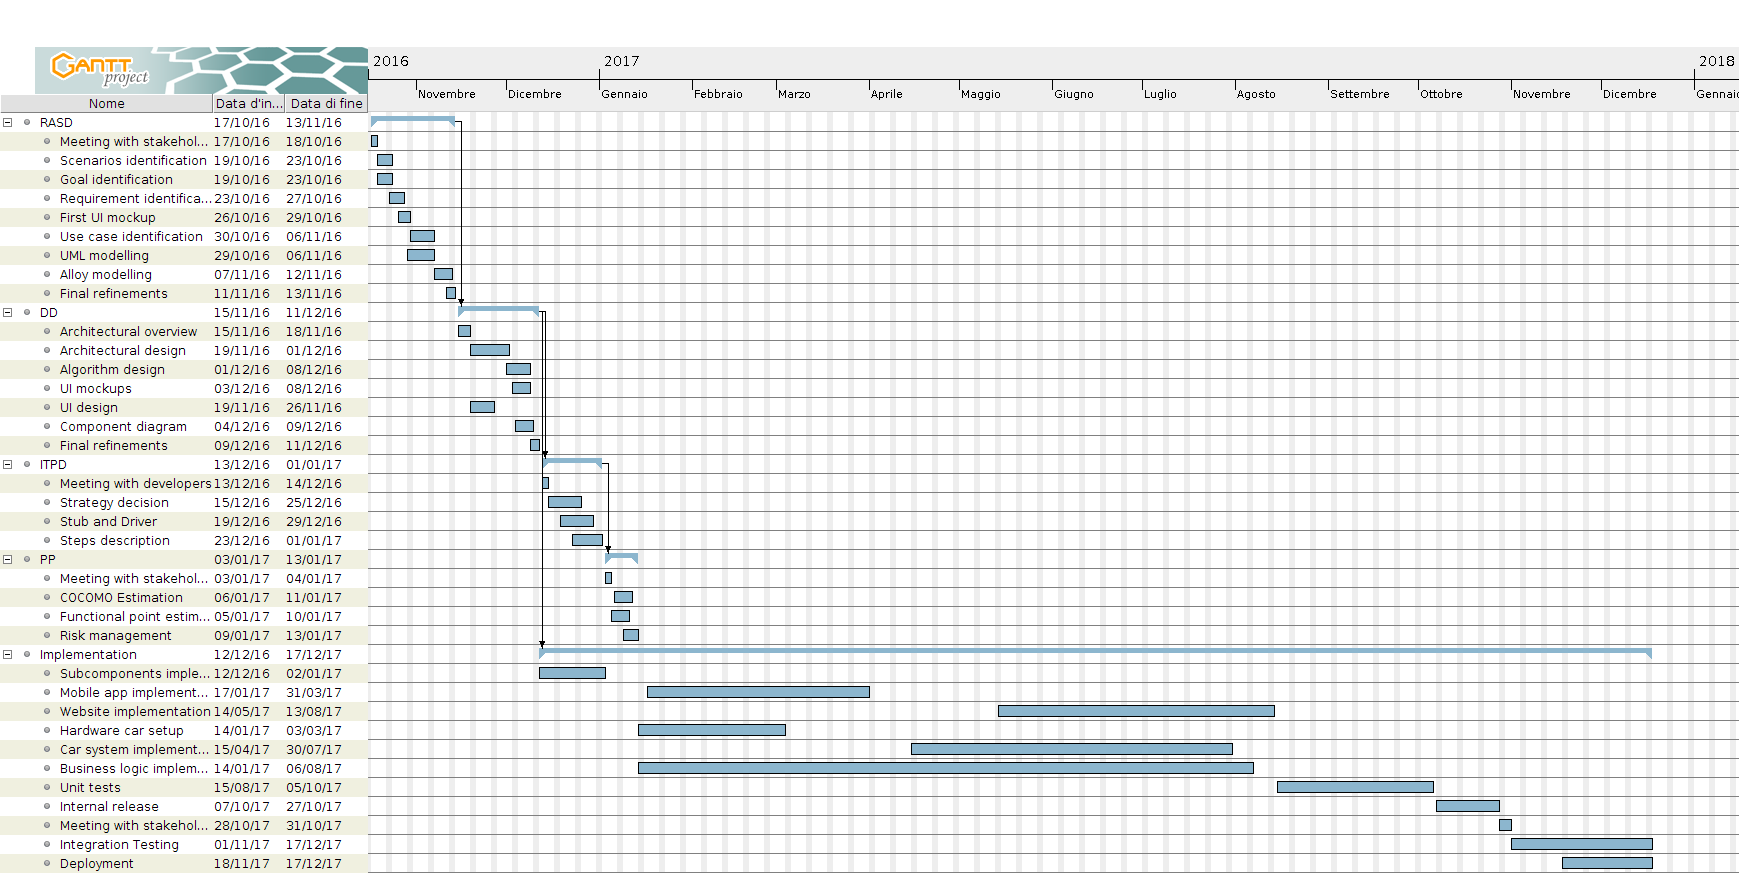
\includegraphics[width=500 pt]{resources/gantt.png}
  \caption{\label{fig:schedule} Gantt diagram for PowerEnJoy project.}
\end{figure}


\newpage
\section{Resource Allocation}
%Anto
Here we will go to define how the tasks are allocated between the three members of the team.
Since our team is composed by homogeneous people, we can consider the same amount of time for each person.

\begin{figure}[h]
  \centering
  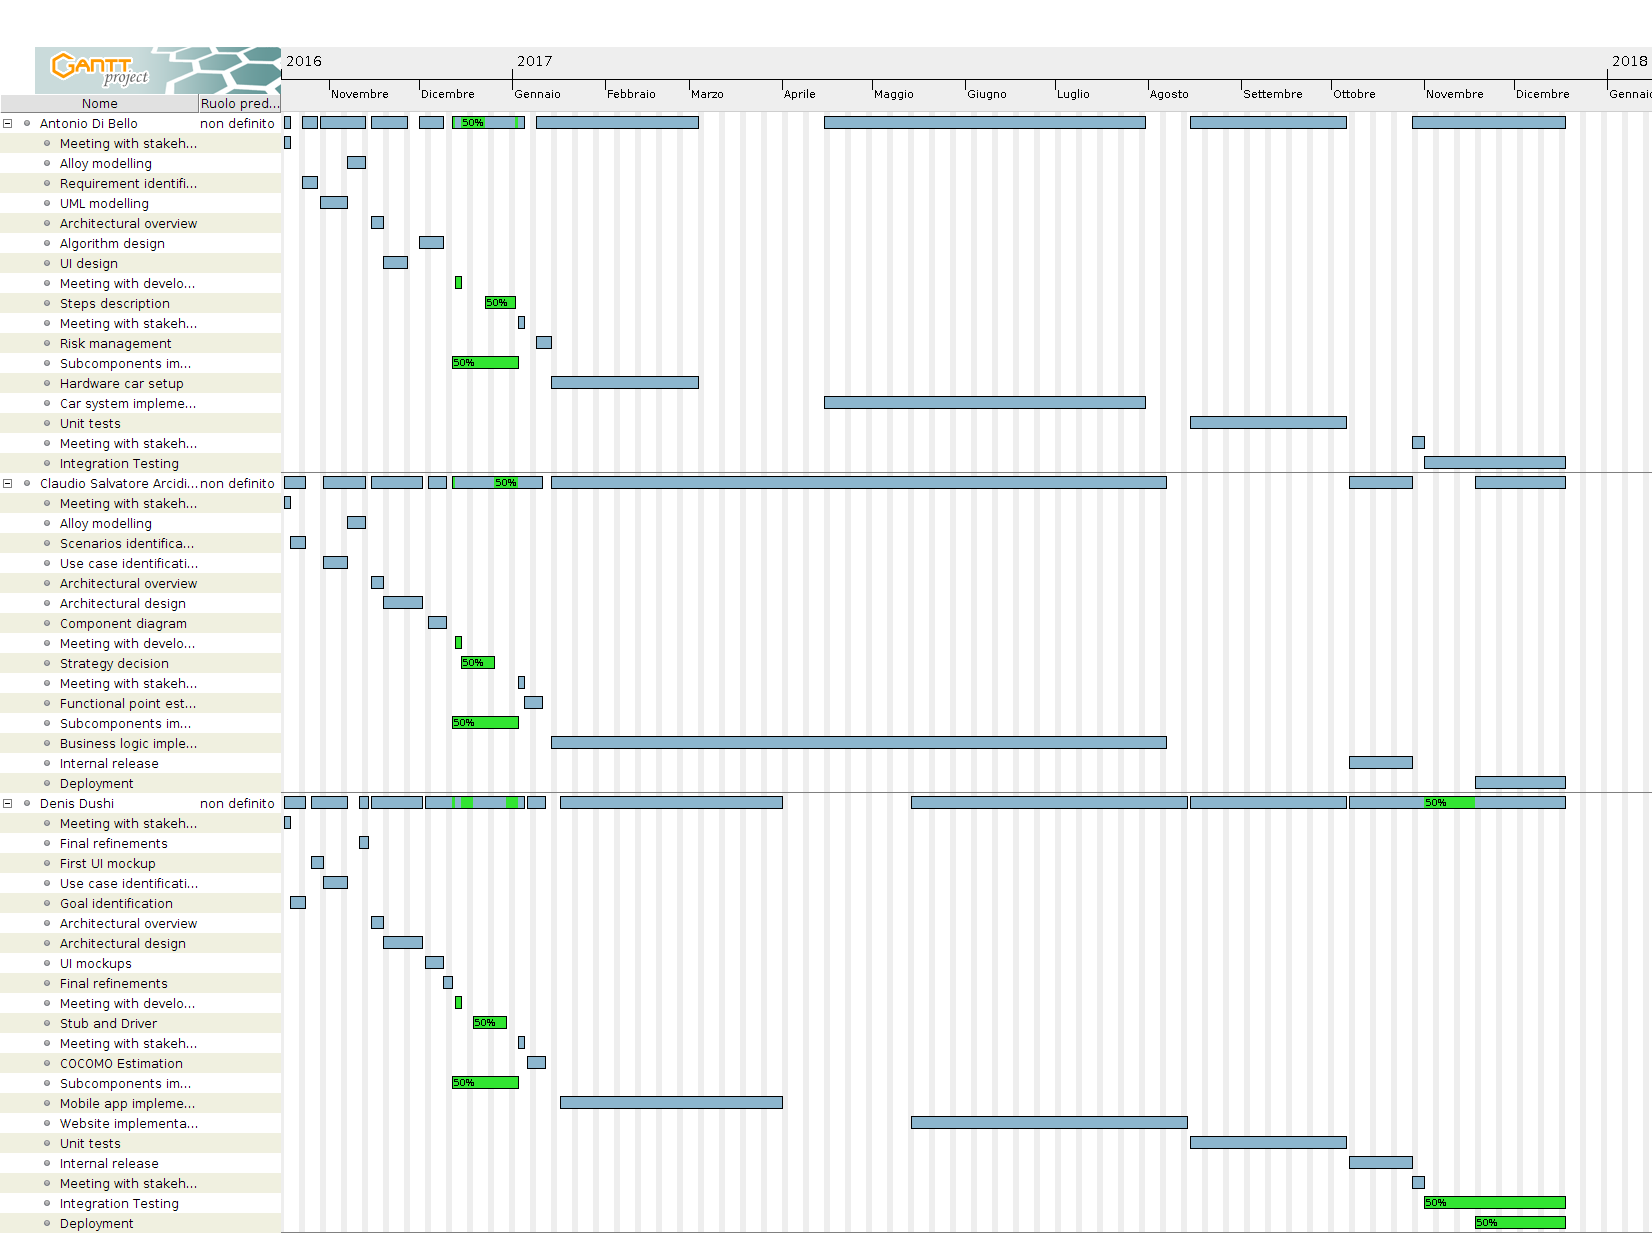
\includegraphics[width=500 pt]{resources/res.png}
  \caption{\label{fig:resource} Resource allocation for each task.}
\end{figure}


\newpage
\section{Risks management}
In this section we are going to explain which are the risks that could affect the realization of our project.
Threats could derive from technical issues, from a wrong business analysis or could be related to controversies with our stakeholders.
For each risk we are going to estimate the probability of occurrence and we will provide a possible contingency plan.\\
The first risk that could jeopardize the project comes from aggressive competition. The competitors that provide a car-sharing service are few but consolidated, therefore they could try to initiating a price war in order to discourage new entrants. The probability that this occurs is high and, without the right precautions, this would affect enormously our business. This risk can be mitigated with a good marketing strategy, in particular is necessary to promote our competitive advantage (electric cars and eco-friendly behaviors) in order to differentiate from competitors.\\
Another potential issue could come from the lack of free space where to build the charging stations or from social movements that protest against the realization of charging stations in cultural areas. In both the cases to overcome the problem we have to make clear to the city administration the advantages that PowerEnJoy provides to the local community and to let the stakeholders have an active role in the development of the project through periodical meetings and demonstrations.\\
Other issues that could be critical have an internal origin : key members of the development team could be ill in periods relevant for the project realization or they could just quit the company. This could lead to delays and a lack of knowledge related to a part of the project. To avoid so it's important to maintain a high quality documentation and to organize the team work assuring that duties and responsibilities are assigned across multiple team members so no critical task is assigned to a single person.\\
We have also to consider the possibility that we underestimate the development time necessary to completely develop the project. In this case allocating new budged in order to add manpower to the project is not recommended, if done in a late phase of development would increase even more the delay! Instead is fundamental to promptly alert the customer of the possible delay and possibly accord on a two-phase release in order to provide as soon as possible a working system and later to add and refine functionalities.\\
Other risks might arise from technical issues that could threat the quality of the product and increase the costs of the software developing process.
The application might have security issues if not well designed. This could lead to a leak of users' sensible data that would be catastrophic for PowerEnJoy's image and therefore for the business of the company. In this case we have to follow all the security standards and test very well the most critical parts to lower as much as possible the probability of occurrence.\\
Other risks that should be considered are related to our dependency on external components. The first suppliers of PowerEnJoy are electric cars vendors. The cars must have a centralized system to provide the possibility to lock/unlock doors remotely. Vendors could try to set inconvenient pricing plans for this additional feature. In this case, since PowerEnJoy needs a large amount of cars, we should leverage on the economy of scale to have lower prices.
Other components that have to be acquired externally are the car displays but this shouldn't be an issue due to the large presence of similar devices in the market.



\newpage
\section{Effort spent}
During the whole project the team worked with the following schedule:\\ \emph{\\}
\textbf{Claudio Salvatore Arcidiacono}
\begin{itemize}
\item 17 January  : 16.30-18.30 2 hours
\item 18 January : 15-20 5 hours
\item 19 January : 17-21 4 hours
\item 20 January : 10-13 3 hours
\item 21 January : 17-20 3 hours 

\textbf{Total hours:} 17 hours.
\end{itemize}


\textbf{Antonio Di Bello}
\begin{itemize}
\item 20 January :  1 hours
\item 21 January :  6 hours
\item 22 January :  3 hours\\

\textbf{Total hours:} 10 hours.
\end{itemize}


\textbf{Denis Dushi}

\begin{itemize}
\item 16 January  :  2 hours
\item 17 January :  2 hours
\item 19 January :  7 hours
\item 20 January :  6 hours
\item 21 January :  5 hours
\item 22 January :  1 hour\\

\textbf{Total hours:} 23 hours.
\end{itemize}

\newpage
\section{References}
\subsection{Software and tool used}
The tools we used to create this document are:
\begin{itemize}
\item Overleaf (for latex writing in parallel)
\end{itemize}

\end{document}